\documentclass[journal, 11pt]{IEEEtran}

\usepackage{epsfig,rotating,setspace,latexsym,amsmath,epsf,amssymb,bm,amsbsy}
\usepackage{cite,graphicx,color,subfigure,here}
\usepackage{amsmath}
\usepackage[normalem]{ulem} 
\usepackage{algorithm}
\usepackage[noend]{algpseudocode}
\usepackage{epstopdf}
\usepackage{scrextend}
\usepackage{ifpdf}
\usepackage{authblk}
\usepackage{caption2}
\usepackage{caption3}
\usepackage[english]{babel}
\usepackage{dsfont}
\usepackage{hyperref}
\providecommand{\keywords}[1]{\textbf{\textit{Index terms---}} #1}

\newcommand{\ba}{\begin{align}}
\newcommand{\ea}{\end{align}}


\begin{document}
\title{Connected Vehicles: Cognition Saves Lives}

\author{Bengi Aygun$^\dag$, Mahni Shayganfar$^*$, and Alexander M.
Wyglinski$^\dag$\\
\normalsize $^\dag$Department of Electrical and Computer Engineering, Worcester
Polytechnic Institute, Worcester, MA\\
\normalsize $^*$Department of Computer Science, Worcester Polytechnic Institute,
Worcester, MA\\
\normalsize Email: \{baygun, alexw\}@wpi.edu, mshayganfar@wpi.edu}

\maketitle

\begin{abstract}
The idea of autonomous cars and connected vehicles is becoming more and more
pervasive in research labs and car manufacturing companies. It is inevitable
that the roads are going to accommodate autonomous and semi-autonomous vehicles
in a near future. However, like other technologies infiltrating into humans
daily life, the transition from conventional transportation systems to
autonomous vehicles requires careful involvement of human-oriented factors into
related technologies. We believe employing cognition in vehicular decision
making processes, improves the awareness and consequently safety and comfort in
the roads. Here, we discuss how affect-driven integration of cognition into
connected vehicles can do so.
\end{abstract}

\begin{keywords}
Cognition, Awareness, Connected Vehicles.
\end{keywords}%

\IEEEpeerreviewmaketitle

\section{Become Connected, Become Aware}

In 1999, the United States Federal Communication Commission (FCC) reserved
$75$~MHz spectrum consisting 6 channels in the $5.9$~GHz band for dedicated
short-range communications (DSRC), which is used for connected vehicle
communications. In February~2014, the National Highway Traffic Safety
Administration (NHTSA) announced that Intelligent Transportation Systems (ITS),
including connected vehicle technology, will be required in all cars by
2019~\cite{factsheet}. Subsequently, there has been a significant increase in
research activities with respect to on vehicular networks (VANETs) as a result
of this urgent need to address vehicular traffic safety concerns~\cite{ntsb}.
The information flow within a connected vehicle network, which includes both
vehicle-to-vehicle (V2V) and vehicle-to-infrastructure (V2I), is managed via the
broadcasting of control messages over a control channel. In Europe, these
messages are referred to Cooperative Awareness Messages (CAMs) while in the
United States they are called Basic Safety Messages (BSMs). Shared information,
such as vehicle position, motion characteristics, and vehicle size, are used for
increasing the overall environmental awareness in support of \textit{safety
applications,} (\textit{e.g.,} intersection movement assist, left turn assist,
do not pass warning sign, and light violation warning) as well as
\textit{mobility applications,} (\textit{e.g.,} collision warning, road
coefficient of friction, road conditions, parking management, and payment
solutions)~\cite{hardingNHTSA14}.

Self and fully autonomous vehicles serve a purpose of traffic safety by
preventing human-driven mistakes. One of the mainstream trials on autonomous
vehicles are performed by Google and Ford Fusion while Volvo and Honda work on
increase the awareness through providing robust device connectivity in vehicular
environment. Connected vehicles stands as a breakthrough on intelligent
transportation while bringing some technological challenges at the same time. In
order to enable robust and efficient ITS mechanisms, several technical
challenges associated with autonomous vehicles include the following:

\begin{itemize}
\item Human-driven mistakes confront autonomous systems with unexpected
situations that makes predefined decision mechanisms insufficient
\item Dynamic vehicular environment includes highly time-varying obstacles,
number of vehicles, and road topology
\item Decision making mechanisms on ITS are not delay-tolerant since the network
environment changes rapidly
\item Periodically broadcasting between connected vehicles causes information
overhead on computer processing unit at each vehicle\\
\end{itemize}

Some research groups are two sides of the same coin but taking this vital
technology one step further by adding a promising functionality:
\textit{Cognition}. Toyota Group currently announced that they investigate
\$$50~M$ to design and produce artificial intelligence within vehicular networks
~\cite{toyota50M}. \textit{Cognition in vehicles assures learn, drive, repair
and socialize with a driver, occupants and other vehicles}~\cite{cogcar}.
Moreover, the driver or passenger's thoughts and habits will be linked to
decision processes. This feature provides a solution to the transition process
from full human driven to half autonomous and half human driven, and finally to
fully autonomous vehicle traffic on roads.

We believe cognition in connected vehicles can:

\begin{itemize}
  \item reduce the amount of errors in the roads caused by drivers, since not
  only autonomous cars drive based on more accurate perception, but also they
  include the behavior model of their neighbors before making any decision,
  \item reduce the amount of required communication since the autonomous cars
  only require to transfer high level decisions based on their own sensory
  information instead of an enormous amount of low level sensory data,
  \item improve the quality of travelling in the roads in terms of safety and
  comfort, since cognition increases awareness of each autonomous vehicle in the
  road.
\end{itemize} 

\section{Cognition in Connected Vehicles}

\subsection{Building Blocks of A Connected Vehicle}

Hardware components shape the technical practicability and readiness of ITS
solutions~\cite{hardingNHTSA14}. Proposed cognition paradigm uses only the
existing components without requiring extra functionality. The intra-vehicle
components are categorized in six main blocks as shown in
Figure~\ref{fig:invehComp}. According to current vision, the internal vehicle
components include two DSRC radios, whose standardization is still under
development. One proposal is to dedicate one radio permanently to safety
messages. An alternative one is to design a multi-channel hopping algorithm to
adaptive use the radios. These radios provide the information sharing with the
other ITS members to increase the awareness.

Another vital component for cognition in vehicles is Global Positioning System
(GPS) receiver for gathering position and timekeeping information. A computer
processing unit use this information with the data generated from onboard
sensors such as heading, speed, acceleration to provide the information to
intra- and inter- vehicles intelligence systems. Safety application electronic
control unit prepares BSMs to periodically broadcast in order to run the safety
applications. Memory unit satisfies the need of data acquisition system; as well
record the historical data on the cognition of its own and other vehicles.
Memory capability also provides a solution to store security certificates.
Lastly, a driver-vehicle interface would be essential for issuing warnings to
the driver. Such warnings could be audible, visual, or haptic, \textit{e.g.,}
tightening of the seat belt, vibrating the driver's seat.

\begin{figure}[!t]
\centerline{\epsfig{figure =figs/car.eps, height=2 in}}
\vspace{-5pt}
\caption{Intra-vehicle components can be used for
cognition~\cite{hardingNHTSA14}.}\label{fig:invehComp}
\vspace{-15pt}
\end{figure}

\subsection{Roads as Social Environments}

A social environment refers to an individual's physical surroundings, resources
and social relationships. A social relationship includes the interaction between
two or more individuals in the environment. A social relationship is the most
dynamic part of a social environment. Hence, developing and maintaining positive
social relationships is crucial for a social environment and is influenced by
the individuals' quality of interaction. Roads are social environments in which
individual vehicles interact with each other through their ``nonverbal"
behaviors obeying the same traffic law. However, there are many violations of
the laws on the roads all over the world in daily basis which consequently leads
to expensive and sorrowful failures. What causes these failures is mostly the
failure of the drivers to effectively interpret their driving environment and
make an appropriate decision with respect to their constraints such as lack of
time, lack of perception, and plethora of cognitive load. Therefore, it is
crucial to involve awareness in the vehicles to share the meaning of what they
dynamically perceive rather than broadcasting the data coming from their sensory
system. For example, any sensory information leading to an alert on a particular
vehicle does not necessarily have the same meaning both for the occupants and
the neighbors of that vehicle. The alert warns the occupants of the vehicle to
be aware of an internal failure (e.g., malfunction in the transmission system),
or an external adversary (e.g., an unexpected leaping of an animal into the
road). The same alert has a different meaning for the close vehicle approaching
from behind; no matter what caused the alert in the leading vehicle, the
posterior vehicle should slow down effective immidiately. However, the same
alert can be interpreted in a totally different way for a neighbor in front of
the originally alerted vehicle. In fact, this vehicle can ignore the received
alert and continue the safe drive. Ultimately, these type of improvements leads
to a higher quality of vehicles' interaction which consequently increases the
safety of the roads.

\subsection{Driving Needs Pareto Optimal Decisions}

Cognitive architectures are used to solve high-dimensional multi-objective
tasks and to make proper decisions with respect to the dynamics of such
environments. Most of the time the real world problems possess a high level of
complexity due to the dynamism involved in the environment. A social environment
is an example of such complex environments. A social environment includes humans
as variety of sources making decisions independently but interrelated to each
other. Roads are social environments and driving is the social act of drivers'
behavior. It is clear that driving involves many decisions in which a driver
needs to maintain its own objectives while recognizing objectives of the others.

\begin{figure}[tbh]
  \centering
  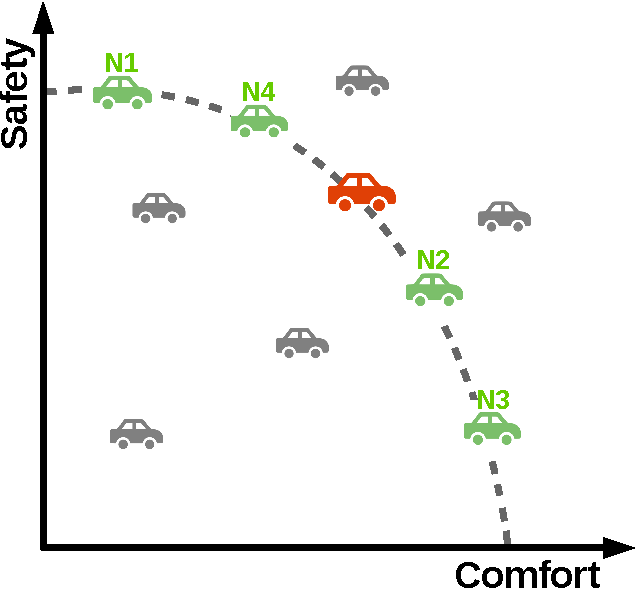
\includegraphics[width=0.35\textwidth]{figs/pareto-croped.pdf}
  \caption{{\fontsize{10}{10}\selectfont Pareto optimal decisions for the
  neighbors.}}
  \label{fig:pareto}
\end{figure}

Let's consider two general objectives, \textit{Safety} and \textit{Comfort}, for
any driver while driving between the source and the destination. Indeed, all the
drivers would like to maximize both of these objectives. However, while they
need to obey the traffic law, they need to take into account their neighbors'
driving behaviors, and respect their objectives. In the example shown in Figure
\ref{fig:pareto}, the red car's driver wants to maximize her own safety and
comfort to her aspiration level for both objectives to obtain the ``preferred''
point. We believe at least for certain redius, the red vehicle should consider
objectives of the other vehicles in that neighborhood (four vehicles shown in
green), and update their anticipated and its own state based on their behaviors.
To achieve this goal, a cognitive system should be able to make decisions with
which it is impossible to change the state of self better off without making the
state of at least one of the neighbors worse off. Therefore, the cognitive
system's decision for any given event should be a pareto optimal solution, since
the neighboring connected vehicles' objectives are important for each individual
vehicle. Here, we only used the concept of pareto optimality to discuss the type
of decisions a cognitive system of a vehicle should make. Our cognitive system
and the underlying mechanisms do not take a game theoretic approach to make
decisions.

\section{Cognition Systems}

Integration of cogniton into connected vehicles needs us to understand the
building blocks of cognition, how do they relate to each other, and what
functional operations they provide. We choose Newell's general theory of
cognitive control, PEACTIDM \cite{newell:unified-cognition}, to describle the
underlying abstract processes of a cognitive system. PEACTIDM is a theory of
cognitive control where cognition is decomposed into a set of eight abstract
functional operations \cite{newell:unified-cognition} all of which are
hypothesized as the building blocks of one's immediate behavior. Figure
\ref{fig:peactidm} shows the sequence of PEACTIDM's building blocks.

\textit{Perceive} is the reception of raw sensory data. For instance, connected
vehicles receive data from both their own local sensory system (e.g., GPS) and
their neighbor vehicles (e.g., an abrupt change in their velocities).
\textit{Encode} is the transformation of the sensory data into features that the
cognitive system can process. In the cognitive architectures using Bratman's BDI
paradigm \cite{bratman:intentions-plans} each sensory data will be tranformed
into a new \textit{belief}. The cognitive architecture will be able to use these
beliefs in different processes. For example, in connected vehicles there will be
a belief about the current accelaration value of the vehicle which corresponds
to the sensory data indicating this value. \textit{Attend} is the act of
shifting or maintaining the focus of attention on an event. For instance, an
alert raised because of a sudden speed reduction of multiple leading neighbor
vehicles needs to be attended immediately while the same alert does not need the
same level of attention if the leading vehicles are a few miles apart.
\textit{Comprehend} is the act of trnasforming an event into a goal or
task-spcific representation and inferring the curent status of the world. For
instance, a vehicle receiving an alert requiring an immediate reaction needs to
identify the cause of the problem even though the alert has raised and received
from another vehicle. Thus, the receiver of the alert can apply replanning if
necessary.

\begin{figure}[tbh]
  \centering
  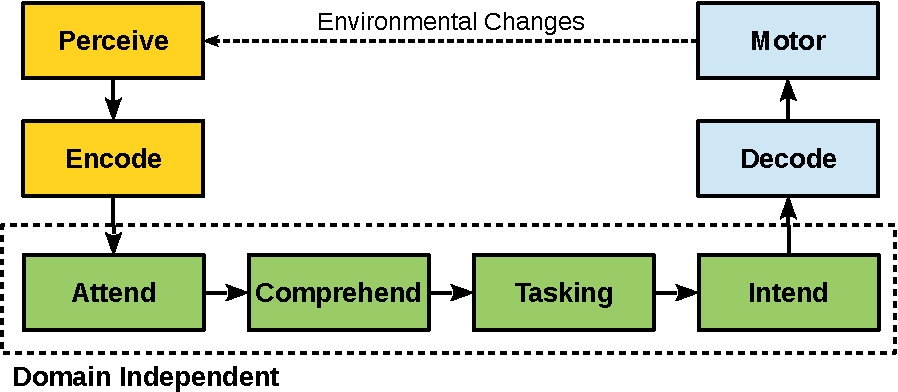
\includegraphics[width=0.485\textwidth]{figs/peactidm-croped.pdf}
  \caption{{\fontsize{10}{10}\selectfont PEACTIDM}}
  \label{fig:peactidm}
\end{figure}

\textit{Tasking} is the process of recognizing a goal based on the new state of
the world. For example, a vehicle can recognize a goal in the plan to exit the
highway with respect to the new beliefs about an accident a few miles ahead and
the current state of the highway which causes constant speed reduction.
\textit{Intend} initiates a future action based on the current goal as response
to the current event. For instance, if the current goal of the vehicle is to
leave the highway, the vehicle begins to change the lane to the right most to be
able to take the next exit. \textit{Decode} translates the response based on the
given \textit{intention} into a series of motor actions. For instance, if the
intention is changing the lane to the right, The vehicle applies a series of
actions including using the right blinker, checking the occupancy status of the
right lane, and turning the steering wheel to the right whenever it is
appropriate. \textit{Motor} executes the actions decoded based on the given
intention. For example, in case of a lane change, the blinker starts to blink
and the wheels turn to the right respective to the amount of change on the
steering wheel.

\section{{\fontsize{11.5}{9}\selectfont Affective Motivational Collaboration
Theory}}
\label{sec:amct}

\textit{Affective Motivational Collaboration Theory}
\cite{shayganfar:theory-overview} is about the interpretation and prediction of
observable behaviors in a dyadic collaborative interaction. Affective
Motivational Collaboration Theory specifies the processes involved in the
progress of a collaboration and how they impact the collaboration's underlying
structure. This theory is built on the foundations of the \textit{SharedPlans}
theory of collaboration \cite{grosz:plans-discourse} and the \textit{cognitive
appraisal} theory of emotions \cite{gratch:domain-independent}.

The theory focuses on the processes regulated by emotional states. It aims to
explain both rapid emotional reactions to events as well as slower, more
deliberative responses. The observable behaviors represent the outcome of
reactive and deliberative processes related to the interpretation of the self's
relationship to the collaborative environment. Affective Motivational
Collaboration Theory aims to explain both rapid emotional reactions to events as
well as slower, more deliberative responses. The reactive and deliberative
processes are triggered by two types of events: \textit{external} events, such
as the other's \textit{nonverbal behaviors} and \textit{primitive actions}, and
\textit{internal} events, comprising changes in the self's mental states, such
as belief formation and emotional changes.

Affective Motivational Collaboration Theory explains how emotions regulate the
underlying processes when these events occur during collaboration. This theory
elucidates the role of motives as goal-driven affect-regulated constructs with
which an agent can form new intentions to cope with internal and external
events. Therefore, a new motive can become a new intention and the self can take
a new action based on the new intention.  The focus of underlying mechanisms is
on the ones depicted as mental processes in Figure \ref{fig:cpm} along with the
mental states.

\begin{figure}[tbh]
  \centering
  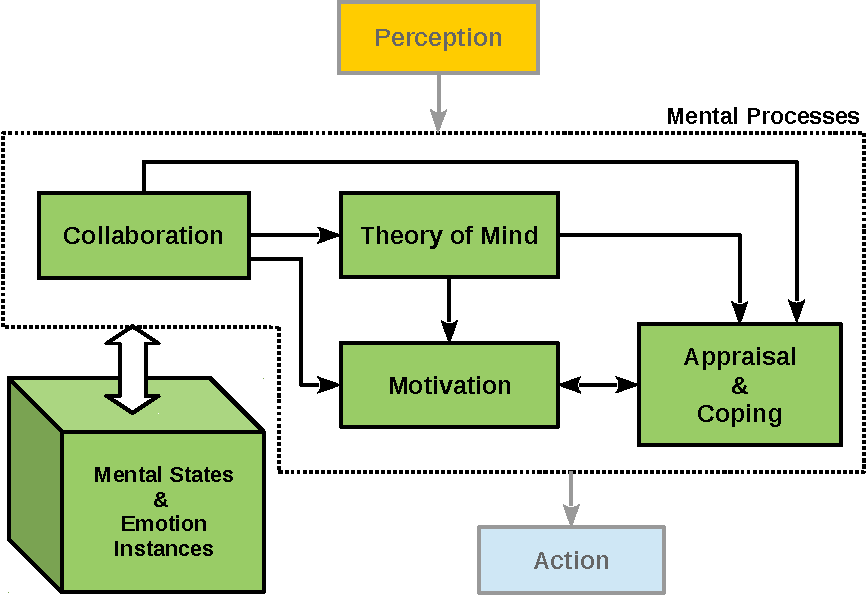
\includegraphics[width=0.485\textwidth]{figs/theory-general-croped.pdf}
  \caption{{\fontsize{10}{10}\selectfont Computational framework based on
  Affective Motivational Collaboration Theory (arrows indicate primary
  influences between mechanisms).}}
  \label{fig:cpm}
\end{figure}

The \textit{Mental States} includes ego's (vehicle's) beliefs, intentions,
motives, goals and emotion instances as well as the anticipated Mental States of
the neighbors (other vehicles). For instance, every sensory data, every
threshold value, or every inferred information about the world has a
corresponding belief in the Mental States. The \textit{Collaboration} mechanism
maintains constraints on actions, including task states and the ordering of
tasks. Although maintaining safety and comfort is a goal for each individual
vehicle, all vehicles also have a shared goal to achieve which is sharing the
road with others -- at least partially -- to get to their destinations.
Therefore, vehicles require a mechanism to maintain their full or partial shared
plan. The \textit{Collaboration} mechanism also provides processes to update and
monitor the shared plan. The \textit{Appraisal} mechanism is responsible for
evaluating changes in the ego's Mental States, the anticipated Mental States of
the neighbors, and the state of the collaboration environment. The outcome of
appraisal impacts every vehicle as an evaluative, regulatory, or motivative
process. For instance, \textit{expectedness} of an event indicates how prepared
is the ego to cope with the event, or how to maintain current state with respect
to the current changes in neighbors' location. The \textit{Coping} mechanism
provides the ego with different coping strategies associated with changes in the
ego's mental states with respect to the state of the collaboration. For
instance, does ego need to change speed with respect to the current state of
the road, or does it need to replan to get to the destination. The
\textit{Motivation} mechanism operates whenever the ego a) requires a new
motive to form a new intention with respect to current event, or b) wants to
interpret a neighbor's motive whenever the neighbor's behavior triggers an
alarm after ego appraising the situation. The \textit{Theory of Mind} mechanism
is the mechanism that infers a model of the neighbor's anticipated mental state.
The ego progressively updates this model during the collaboration. A neighbor's
model impacts ego's decision with respect to the state of the neighbor.

\section{Example Scenario}
\label{sec:example-scenario}

According to the analysis of the lane change by the US' National Highway Traffic
Safety Administration (NHTSA) in 2003 more than 38\% of pre-crash movements in
the highways was caused by typical lane change. Furthermore, according to the
NHTSA's traffic safety facts of February 2015, about the 94\% of the critical
reasons of pre-crashed events are attributed to the drivers. As mentioned in
this report, about 41\% of the driver-related critical reasons are because of
the \textit{\textbf{drivers' recognition errors}} including driver’s
inattention, internal and external distractions, and inadequate surveillance.
Also, about 33\% of pre-crash reasons are caused by the \textit{\textbf{driver's
decision errors}} such as driving too fast for conditions, too fast for the
curve, false assumption of others’ actions, illegal maneuver and misjudgment of
gap or others’ speed. In our hypothetical example, we show how the involvement
of different mechanisms in our framework can improve safety and comfort for both
the ego vehicle and the other neighbor(s) in the roads for such conditions.

\begin{figure}[!t]
  \centerline{\epsfig{figure =figs/ex1.eps, height=1.45 in}}
  \vspace*{-2mm}
  \caption{Being aware of other drivers' intention.}
  \label{fig:example1}
  \vspace*{-5mm}
\end{figure}

In this example (see Figure \ref{fig:example1}), autonomous Vehicle
\textit{A} (ego vehicle) travelling in the right lane wants to take Exit
\textit{x} in two miles. However, the ego vehicle has decided to pass the
slow-moving Truck \textit{D} before taking Exit \textit{x}, since it is late. At
the same time, Vehicle \textit{B}, travelling in the left lane, quickly
approaches a slower car, Vehicle \textit{C} in the same lane. Vehicle
\textit{B}'s driver decides to change lane to the middle lane to pass Vehicle
\textit{C}. Therefore, both the autonomous Vehicle \textit{A} and the driver of
Vehicle \textit{B} want to go to the middle lane at the same time; since the
middle lane is not occupied by any other vehicle. Hence, because both Vehicle
\textit{A} and Vehicle \textit{B} are not aware of each other's intention, they
can cause an accident irrespective of the responsibility of each vehicle with
respect to the traffic law.

In this example, the ego vehicle perceives a sudden change of lane by Vehicle
\textit{B}; then it appraises this event as \textit{relevant, undesirable,
unexpected}, and \textit{controllable}. The lane change by Vehicle \textit{B} is
relevant to ego vehicle since it decreases the utility of the current goal for
the ego vehicle; it is undesirable since the ego vehicle's attempted goal (lane
change) is not achieved (i.e., it is blocked); it is unexpected since the
Vehicle \textit{B} interrupted the ego vehicle pursuing its current goal; and it
is controllable since the ego vehicle still has three alternative goals to
pursue. The goal management process in our framework ranks all of the potential
goals based on their status in the plan structure, and the outcome of the self
and the reverse appraisal. Moreover, in this incident the ego vehicle does not
have a behavior model of the Vehicle \textit{B}, since Vehicle \textit{B} has
just reached to the ego vehicle and is perceived for the first time. Therefore,
first, the ego vehicle replaces the current goal with stay-in-the-lane goal for
the prupose of recovering from the blocked goal. In general, the ego vehicle
adopts one of the safe predefined tactical goals, e.g., stay-in-the-lane or
reduce-speed, as an alternative goal to which pursuing it raises unexpected and
undesirable events. Next, the ego vehicle chooses the \textit{restraint coping
strategy} to immediately pull back into the right lane to yield the the middle
lane to Vehicle \textit{B} avoiding any possible accident. Therefore, choosing
an appropriate coping strategy, the ego vehicle responds to the current goal
change using the sensory system and taking appropriate actions to pursue the new
stay-in-the-lane goal. The ego vehicle updates the Vehicle \textit{B}'s user
model to a reckless driver. As shown in this example, the cognition of the
autonomous vehicle prevented an accident which could happen because of the
drivers' recognition error caused by their inadequate survillance in the
highway.

\begin{figure}[!t]
  \centerline{\epsfig{figure =figs/ex2.eps, height=1.1 in}}
  \vspace*{-2mm}
  \caption{Coping with the driving behavior of a reckless driver.}
  \label{fig:example2}
  \vspace*{-5mm}
\end{figure}

In the next incident (see Figure \ref{fig:example2}), the ego vehicle perceives
Vehicle \textit{B} quickly approaching from behind in the middle lane (event 1).
Vehicle \textit{B} changes its lane to the right lane (instead of left) to pass
the ego vehicle immediately after reaching the ego vehicle (event 2). As
shown in Figure \ref{fig:example2}, Vehicle \textit{B} has to switch back to the
middle lane quickly (event 3), since there is a slow-moving truck in the right
lane at a short distance ahead of the ego vehicle. However, Vehicle \textit{D}
makes another blockage for Vehicle \textit{B} in the middle lane. Consequently,
Vehicle \textit{B} has to switch to the left lane to pass this blockage (event
4). All these four events happen in a few seconds in the neigborhood of the ego
vehicle.

Similar to the first incident, the ego vehicle appraises the first event as
highly \textit{relevant, undesirable, unexpected} and \textit{controllable} for
the self, and \textit{relevant, desirable} and \textit{expected} with low value
of \textit{controllability} for Vehicle \textit{B}. Therefore, the ego Vehicle,
creates a behavior model for Vehicle \textit{B} with a probability of having
a \textit{speeding} driver. The next three events will be also appraised in the
same way. The ego vehicle updates Vehicle \textit{B}'s behavior model based on
each event, raising the probability of Vehicle \textit{B} having a
\textit{speeding} driver. Updating Vehicle \textit{B}'s behvior model based on
several events leads to a more accurate behavior model of Vehicle \textit{B}.
Consequently, the ego vehicle will be able to evaluate Vehicle \textit{B}'s
actions more accurately based on the reverse appraisal process. The outcome of
the self and reverse appraisal processes causes the goal management process to
employ another tactical goal, i.e., reduce-speed. Hence, the ego vehicle as the
outcome of the appraisal and the behavior modeling processess adopts
\textit{behavioral disengagement} as the most appropriate coping strategy.
Furthermore, Vehicle \textit{B}'s behavior model not only helps the ego vehicle
to be safe while travelling in its neighborhood, but it can also inform other
autonomous vehicles to drive carefully while Vehicle \textit{B} is in a short
distance from them.

In the last incident the ego vehicle (Vehcile \textit{A}) simply passes another
autonomous car (Vehicle \textit{B}) which is driving in the right lane with a
normal speed (see Figure \ref{fig:example3}). Vehicle \textit{B} also detects
the appearance of another autonomous vehicle in its own neighborhood. The ego
vehicle receives an alert from Vehicle \textit{B} regarding the car (Vehicle
\textit{C}) travelling a few hundred feet in front of them in the middle lane.
The alert message contains a vector of probabilities of the Vehicle \textit{C}'s
driver type indicating the following probabilities: 34\% chance of being
\textit{drowsy driver}, 32\% of chance of driving \textit{under the influence of
drugs or alcohol}, 28\% chance of being \textit{distracted driver}, and 6\%
chance of being a \textit{teenage driver}. These values are computed by the
Vehicle \textit{B}'s Bayesian behavior modelling process in the the Theory of
Mind mechanism. Comoputing these probability values is based on Vehicle
\textit{B}'s perception and appraisal of the road including the Vehicle
\textit{C}, even before the ego vehicle reaches to Vehicle \textit{B}.
Afterwards, the ego vehicle uses the content of the alert message to update it's
own behavior model of the Vehicle \textit{C}. Updating Vehicle \textit{C}'s
behavior model does not change the ego vehicle's current goal. It also does not
demand the ego vehicle to apply an immediate reactive change in its own driving
behavior. However, it replaces the current motive (i.e., maintain the current
speed) of the ego vehicle with a new motive (i.e., maintain the current distance
with Vehicle \textit{C}). Forming this new motive is based on the outcome of the
Theory of Mind (updated by another vehicle) and the Appraisal mechanisms. The
new motive is urgent since it requires an immediate change in ego vehicle's
driving behavior, and it is important since it is related to the current goal
that the ego vehicle pursues. Therefore, the new motive causes the ego vehicle
to adopt an \textit{active coping strategy} to circumvent the stressor (i.e.,
Vehicle \textit{C}) by maintaining its distance.

\begin{figure}[!t]
  \centerline{\epsfig{figure =figs/ex3.eps, height=1.1 in}}
  \vspace*{-2mm}
  \caption{Communicating the behavior model of careless driver.}
  \label{fig:example3}
  \vspace*{-5mm}
\end{figure}

\section{Conclusion}
\label{Conc}
%

\bibliographystyle{IEEEtran}
\bibliography{mshayganfar,referencesVTM}
% \bibliography{referencesVTM}
\end{document}
